\documentclass[twoside]{book}

% Packages required by doxygen
\usepackage{fixltx2e}
\usepackage{calc}
\usepackage{doxygen}
\usepackage[export]{adjustbox} % also loads graphicx
\usepackage{graphicx}
\usepackage[utf8]{inputenc}
\usepackage{makeidx}
\usepackage{multicol}
\usepackage{multirow}
\PassOptionsToPackage{warn}{textcomp}
\usepackage{textcomp}
\usepackage[nointegrals]{wasysym}
\usepackage[table]{xcolor}

% Font selection
\usepackage[T1]{fontenc}
\usepackage[scaled=.90]{helvet}
\usepackage{courier}
\usepackage{amssymb}
\usepackage{sectsty}
\renewcommand{\familydefault}{\sfdefault}
\allsectionsfont{%
  \fontseries{bc}\selectfont%
  \color{darkgray}%
}
\renewcommand{\DoxyLabelFont}{%
  \fontseries{bc}\selectfont%
  \color{darkgray}%
}
\newcommand{\+}{\discretionary{\mbox{\scriptsize$\hookleftarrow$}}{}{}}

% Page & text layout
\usepackage{geometry}
\geometry{%
  a4paper,%
  top=2.5cm,%
  bottom=2.5cm,%
  left=2.5cm,%
  right=2.5cm%
}
\tolerance=750
\hfuzz=15pt
\hbadness=750
\setlength{\emergencystretch}{15pt}
\setlength{\parindent}{0cm}
\setlength{\parskip}{3ex plus 2ex minus 2ex}
\makeatletter
\renewcommand{\paragraph}{%
  \@startsection{paragraph}{4}{0ex}{-1.0ex}{1.0ex}{%
    \normalfont\normalsize\bfseries\SS@parafont%
  }%
}
\renewcommand{\subparagraph}{%
  \@startsection{subparagraph}{5}{0ex}{-1.0ex}{1.0ex}{%
    \normalfont\normalsize\bfseries\SS@subparafont%
  }%
}
\makeatother

% Headers & footers
\usepackage{fancyhdr}
\pagestyle{fancyplain}
\fancyhead[LE]{\fancyplain{}{\bfseries\thepage}}
\fancyhead[CE]{\fancyplain{}{}}
\fancyhead[RE]{\fancyplain{}{\bfseries\leftmark}}
\fancyhead[LO]{\fancyplain{}{\bfseries\rightmark}}
\fancyhead[CO]{\fancyplain{}{}}
\fancyhead[RO]{\fancyplain{}{\bfseries\thepage}}
\fancyfoot[LE]{\fancyplain{}{}}
\fancyfoot[CE]{\fancyplain{}{}}
\fancyfoot[RE]{\fancyplain{}{\bfseries\scriptsize Generated by Doxygen }}
\fancyfoot[LO]{\fancyplain{}{\bfseries\scriptsize Generated by Doxygen }}
\fancyfoot[CO]{\fancyplain{}{}}
\fancyfoot[RO]{\fancyplain{}{}}
\renewcommand{\footrulewidth}{0.4pt}
\renewcommand{\chaptermark}[1]{%
  \markboth{#1}{}%
}
\renewcommand{\sectionmark}[1]{%
  \markright{\thesection\ #1}%
}

% Indices & bibliography
\usepackage{natbib}
\usepackage[titles]{tocloft}
\setcounter{tocdepth}{3}
\setcounter{secnumdepth}{5}
\makeindex

% Hyperlinks (required, but should be loaded last)
\usepackage{ifpdf}
\ifpdf
  \usepackage[pdftex,pagebackref=true]{hyperref}
\else
  \usepackage[ps2pdf,pagebackref=true]{hyperref}
\fi
\hypersetup{%
  colorlinks=true,%
  linkcolor=blue,%
  citecolor=blue,%
  unicode%
}

% Custom commands
\newcommand{\clearemptydoublepage}{%
  \newpage{\pagestyle{empty}\cleardoublepage}%
}

\usepackage{caption}
\captionsetup{labelsep=space,justification=centering,font={bf},singlelinecheck=off,skip=4pt,position=top}

%===== C O N T E N T S =====

\begin{document}

% Titlepage & ToC
\hypersetup{pageanchor=false,
             bookmarksnumbered=true,
             pdfencoding=unicode
            }
\pagenumbering{alph}
\begin{titlepage}
\vspace*{7cm}
\begin{center}%
{\Large G\+A\+M\+LP \\[1ex]\large 1 }\\
\vspace*{1cm}
{\large Generated by Doxygen 1.8.14}\\
\end{center}
\end{titlepage}
\clearemptydoublepage
\pagenumbering{roman}
\tableofcontents
\clearemptydoublepage
\pagenumbering{arabic}
\hypersetup{pageanchor=true}

%--- Begin generated contents ---
\chapter{Namespace Index}
\section{Namespace List}
Here is a list of all documented namespaces with brief descriptions\+:\begin{DoxyCompactList}
\item\contentsline{section}{\mbox{\hyperlink{namespacesrc}{src}} }{\pageref{namespacesrc}}{}
\end{DoxyCompactList}

\chapter{Hierarchical Index}
\section{Class Hierarchy}
This inheritance list is sorted roughly, but not completely, alphabetically\+:\begin{DoxyCompactList}
\item Exception\begin{DoxyCompactList}
\item \contentsline{section}{src.\+operator\+\_\+gen.\+Bad\+Script}{\pageref{classsrc_1_1operator__gen_1_1BadScript}}{}
\end{DoxyCompactList}
\item \contentsline{section}{src.\+solvers.\+Method}{\pageref{classsrc_1_1solvers_1_1Method}}{}
\item \contentsline{section}{src.\+node.\+Node}{\pageref{classsrc_1_1node_1_1Node}}{}
\begin{DoxyCompactList}
\item \contentsline{section}{src.\+equation.\+Equation}{\pageref{classsrc_1_1equation_1_1Equation}}{}
\item \contentsline{section}{src.\+intnode.\+Int\+Node}{\pageref{classsrc_1_1intnode_1_1IntNode}}{}
\item \contentsline{section}{src.\+operatornode.\+Operator\+Node}{\pageref{classsrc_1_1operatornode_1_1OperatorNode}}{}
\begin{DoxyCompactList}
\item \contentsline{section}{src.\+operators.\+Div\+Node}{\pageref{classsrc_1_1operators_1_1DivNode}}{}
\item \contentsline{section}{src.\+operators.\+Homogen\+Operator}{\pageref{classsrc_1_1operators_1_1HomogenOperator}}{}
\begin{DoxyCompactList}
\item \contentsline{section}{src.\+operators.\+Add\+Node}{\pageref{classsrc_1_1operators_1_1AddNode}}{}
\item \contentsline{section}{src.\+operators.\+Mul\+Node}{\pageref{classsrc_1_1operators_1_1MulNode}}{}
\end{DoxyCompactList}
\item \contentsline{section}{src.\+operators.\+Pow\+Node}{\pageref{classsrc_1_1operators_1_1PowNode}}{}
\item \contentsline{section}{src.\+operators.\+Sub\+Node}{\pageref{classsrc_1_1operators_1_1SubNode}}{}
\end{DoxyCompactList}
\item \contentsline{section}{src.\+unitnode.\+Unit\+Node}{\pageref{classsrc_1_1unitnode_1_1UnitNode}}{}
\item \contentsline{section}{src.\+varnode.\+Var\+Node}{\pageref{classsrc_1_1varnode_1_1VarNode}}{}
\end{DoxyCompactList}
\item \contentsline{section}{src.\+operator\+\_\+gen.\+Operator}{\pageref{classsrc_1_1operator__gen_1_1Operator}}{}
\item \contentsline{section}{src.\+solvers.\+Solver}{\pageref{classsrc_1_1solvers_1_1Solver}}{}
\end{DoxyCompactList}

\chapter{Class Index}
\section{Class List}
Here are the classes, structs, unions and interfaces with brief descriptions\+:\begin{DoxyCompactList}
\item\contentsline{section}{\mbox{\hyperlink{classsrc_1_1operators_1_1AddNode}{src.\+operators.\+Add\+Node}} }{\pageref{classsrc_1_1operators_1_1AddNode}}{}
\item\contentsline{section}{\mbox{\hyperlink{classsrc_1_1operator__gen_1_1BadScript}{src.\+operator\+\_\+gen.\+Bad\+Script}} }{\pageref{classsrc_1_1operator__gen_1_1BadScript}}{}
\item\contentsline{section}{\mbox{\hyperlink{classsrc_1_1operators_1_1DivNode}{src.\+operators.\+Div\+Node}} }{\pageref{classsrc_1_1operators_1_1DivNode}}{}
\item\contentsline{section}{\mbox{\hyperlink{classsrc_1_1equation_1_1Equation}{src.\+equation.\+Equation}} }{\pageref{classsrc_1_1equation_1_1Equation}}{}
\item\contentsline{section}{\mbox{\hyperlink{classsrc_1_1operators_1_1HomogenOperator}{src.\+operators.\+Homogen\+Operator}} }{\pageref{classsrc_1_1operators_1_1HomogenOperator}}{}
\item\contentsline{section}{\mbox{\hyperlink{classsrc_1_1intnode_1_1IntNode}{src.\+intnode.\+Int\+Node}} }{\pageref{classsrc_1_1intnode_1_1IntNode}}{}
\item\contentsline{section}{\mbox{\hyperlink{classsrc_1_1solvers_1_1Method}{src.\+solvers.\+Method}} }{\pageref{classsrc_1_1solvers_1_1Method}}{}
\item\contentsline{section}{\mbox{\hyperlink{classsrc_1_1operators_1_1MulNode}{src.\+operators.\+Mul\+Node}} }{\pageref{classsrc_1_1operators_1_1MulNode}}{}
\item\contentsline{section}{\mbox{\hyperlink{classsrc_1_1node_1_1Node}{src.\+node.\+Node}} }{\pageref{classsrc_1_1node_1_1Node}}{}
\item\contentsline{section}{\mbox{\hyperlink{classsrc_1_1operator__gen_1_1Operator}{src.\+operator\+\_\+gen.\+Operator}} }{\pageref{classsrc_1_1operator__gen_1_1Operator}}{}
\item\contentsline{section}{\mbox{\hyperlink{classsrc_1_1operatornode_1_1OperatorNode}{src.\+operatornode.\+Operator\+Node}} }{\pageref{classsrc_1_1operatornode_1_1OperatorNode}}{}
\item\contentsline{section}{\mbox{\hyperlink{classsrc_1_1operators_1_1PowNode}{src.\+operators.\+Pow\+Node}} }{\pageref{classsrc_1_1operators_1_1PowNode}}{}
\item\contentsline{section}{\mbox{\hyperlink{classsrc_1_1solvers_1_1Solver}{src.\+solvers.\+Solver}} }{\pageref{classsrc_1_1solvers_1_1Solver}}{}
\item\contentsline{section}{\mbox{\hyperlink{classsrc_1_1operators_1_1SubNode}{src.\+operators.\+Sub\+Node}} }{\pageref{classsrc_1_1operators_1_1SubNode}}{}
\item\contentsline{section}{\mbox{\hyperlink{classsrc_1_1unitnode_1_1UnitNode}{src.\+unitnode.\+Unit\+Node}} }{\pageref{classsrc_1_1unitnode_1_1UnitNode}}{}
\item\contentsline{section}{\mbox{\hyperlink{classsrc_1_1varnode_1_1VarNode}{src.\+varnode.\+Var\+Node}} }{\pageref{classsrc_1_1varnode_1_1VarNode}}{}
\end{DoxyCompactList}

\chapter{Namespace Documentation}
\hypertarget{namespacesrc}{}\section{src Namespace Reference}
\label{namespacesrc}\index{src@{src}}


\subsection{Detailed Description}
\begin{DoxyVerb}@package gamlp
Main pkg
\end{DoxyVerb}
 
\chapter{Class Documentation}
\hypertarget{classsrc_1_1operators_1_1AddNode}{}\section{src.\+operators.\+Add\+Node Class Reference}
\label{classsrc_1_1operators_1_1AddNode}\index{src.\+operators.\+Add\+Node@{src.\+operators.\+Add\+Node}}
Inheritance diagram for src.\+operators.\+Add\+Node\+:\begin{figure}[H]
\begin{center}
\leavevmode
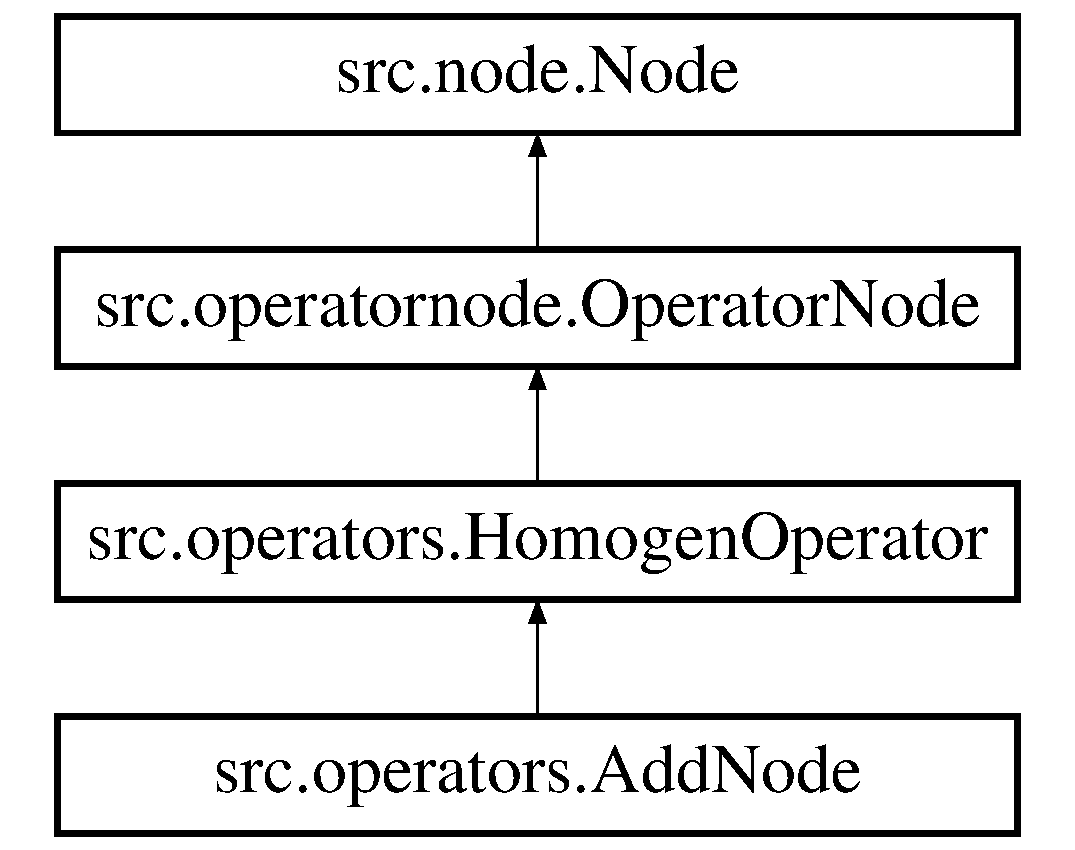
\includegraphics[height=4.000000cm]{classsrc_1_1operators_1_1AddNode}
\end{center}
\end{figure}
\subsection*{Public Member Functions}
\begin{DoxyCompactItemize}
\item 
\mbox{\Hypertarget{classsrc_1_1operators_1_1AddNode_a5f98463a5345ae272d0d5a96193abd05}\label{classsrc_1_1operators_1_1AddNode_a5f98463a5345ae272d0d5a96193abd05}} 
def {\bfseries \+\_\+\+\_\+init\+\_\+\+\_\+} (self, terms)
\item 
\mbox{\Hypertarget{classsrc_1_1operators_1_1AddNode_a9aba65294be7ca5bca93fa80f5226c9b}\label{classsrc_1_1operators_1_1AddNode_a9aba65294be7ca5bca93fa80f5226c9b}} 
def {\bfseries eval} (self)
\item 
\mbox{\Hypertarget{classsrc_1_1operators_1_1AddNode_a6cd89d4e0a8075d51827c45db80c736a}\label{classsrc_1_1operators_1_1AddNode_a6cd89d4e0a8075d51827c45db80c736a}} 
def {\bfseries merge\+\_\+two} (self, term, node)
\item 
\mbox{\Hypertarget{classsrc_1_1operators_1_1AddNode_aadc2111ae48380bed5a886bdf57a7faa}\label{classsrc_1_1operators_1_1AddNode_aadc2111ae48380bed5a886bdf57a7faa}} 
def {\bfseries simplifyed} (self)
\item 
\mbox{\Hypertarget{classsrc_1_1operators_1_1AddNode_a28e3202028869da3f73398cf6e12356f}\label{classsrc_1_1operators_1_1AddNode_a28e3202028869da3f73398cf6e12356f}} 
def {\bfseries latex} (self)
\end{DoxyCompactItemize}
\subsection*{Additional Inherited Members}


The documentation for this class was generated from the following file\+:\begin{DoxyCompactItemize}
\item 
src/operators.\+py\end{DoxyCompactItemize}

\hypertarget{classsrc_1_1operator__gen_1_1BadScript}{}\section{src.\+operator\+\_\+gen.\+Bad\+Script Class Reference}
\label{classsrc_1_1operator__gen_1_1BadScript}\index{src.\+operator\+\_\+gen.\+Bad\+Script@{src.\+operator\+\_\+gen.\+Bad\+Script}}
Inheritance diagram for src.\+operator\+\_\+gen.\+Bad\+Script\+:\begin{figure}[H]
\begin{center}
\leavevmode
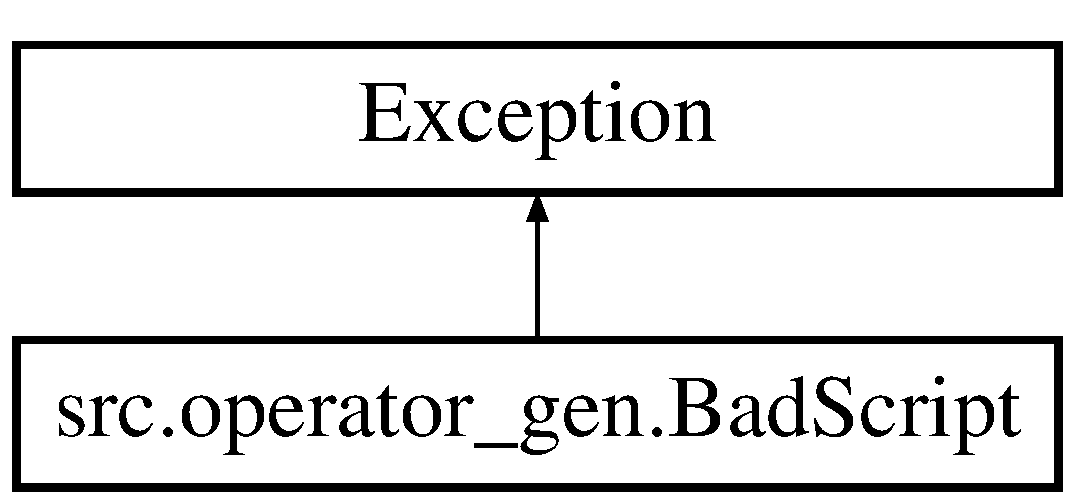
\includegraphics[height=2.000000cm]{classsrc_1_1operator__gen_1_1BadScript}
\end{center}
\end{figure}


The documentation for this class was generated from the following file\+:\begin{DoxyCompactItemize}
\item 
src/operator\+\_\+gen.\+py\end{DoxyCompactItemize}

\hypertarget{classsrc_1_1operators_1_1DivNode}{}\section{src.\+operators.\+Div\+Node Class Reference}
\label{classsrc_1_1operators_1_1DivNode}\index{src.\+operators.\+Div\+Node@{src.\+operators.\+Div\+Node}}
Inheritance diagram for src.\+operators.\+Div\+Node\+:\begin{figure}[H]
\begin{center}
\leavevmode
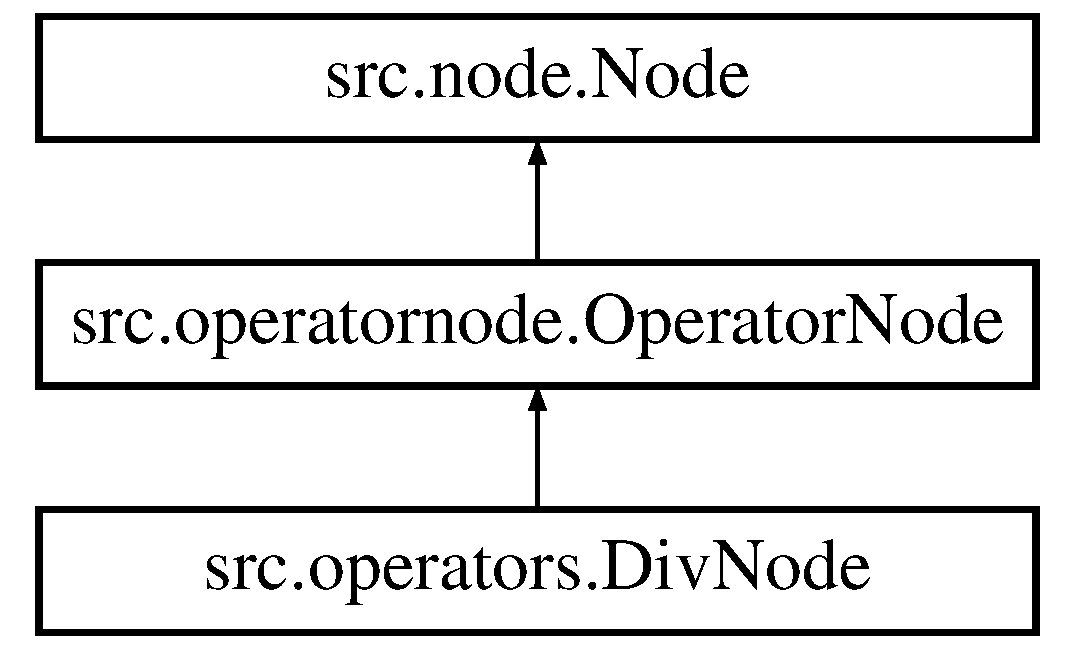
\includegraphics[height=3.000000cm]{classsrc_1_1operators_1_1DivNode}
\end{center}
\end{figure}
\subsection*{Public Member Functions}
\begin{DoxyCompactItemize}
\item 
\mbox{\Hypertarget{classsrc_1_1operators_1_1DivNode_a618b29150f6e15eac331056cf4703d34}\label{classsrc_1_1operators_1_1DivNode_a618b29150f6e15eac331056cf4703d34}} 
def {\bfseries \+\_\+\+\_\+init\+\_\+\+\_\+} (self, left, right)
\item 
\mbox{\Hypertarget{classsrc_1_1operators_1_1DivNode_a3cde8c782f68447da994d02b558e5d82}\label{classsrc_1_1operators_1_1DivNode_a3cde8c782f68447da994d02b558e5d82}} 
def {\bfseries \+\_\+\+\_\+hash\+\_\+\+\_\+} (self)
\item 
\mbox{\Hypertarget{classsrc_1_1operators_1_1DivNode_ada459a6474c88d4fffa3df7400ebe6ae}\label{classsrc_1_1operators_1_1DivNode_ada459a6474c88d4fffa3df7400ebe6ae}} 
def {\bfseries eval} (self)
\item 
\mbox{\Hypertarget{classsrc_1_1operators_1_1DivNode_abf8b2433bf8f33515564ca51c4e17940}\label{classsrc_1_1operators_1_1DivNode_abf8b2433bf8f33515564ca51c4e17940}} 
def {\bfseries formatted} (self)
\item 
\mbox{\Hypertarget{classsrc_1_1operators_1_1DivNode_aa43e51a045b501e045273df03aebc42b}\label{classsrc_1_1operators_1_1DivNode_aa43e51a045b501e045273df03aebc42b}} 
def {\bfseries get\+\_\+children} (self)
\item 
\mbox{\Hypertarget{classsrc_1_1operators_1_1DivNode_a80be77f9cc16d87b3e0648695319562f}\label{classsrc_1_1operators_1_1DivNode_a80be77f9cc16d87b3e0648695319562f}} 
def {\bfseries latex} (self)
\end{DoxyCompactItemize}
\subsection*{Public Attributes}
\begin{DoxyCompactItemize}
\item 
\mbox{\Hypertarget{classsrc_1_1operators_1_1DivNode_a17a585bdb1c142f96c6a33e8b10d8c68}\label{classsrc_1_1operators_1_1DivNode_a17a585bdb1c142f96c6a33e8b10d8c68}} 
{\bfseries left}
\item 
\mbox{\Hypertarget{classsrc_1_1operators_1_1DivNode_a41478d41b14a99f83c1cf56971635ee0}\label{classsrc_1_1operators_1_1DivNode_a41478d41b14a99f83c1cf56971635ee0}} 
{\bfseries right}
\end{DoxyCompactItemize}


The documentation for this class was generated from the following file\+:\begin{DoxyCompactItemize}
\item 
src/operators.\+py\end{DoxyCompactItemize}

\hypertarget{classsrc_1_1equation_1_1Equation}{}\section{src.\+equation.\+Equation Class Reference}
\label{classsrc_1_1equation_1_1Equation}\index{src.\+equation.\+Equation@{src.\+equation.\+Equation}}
Inheritance diagram for src.\+equation.\+Equation\+:\begin{figure}[H]
\begin{center}
\leavevmode
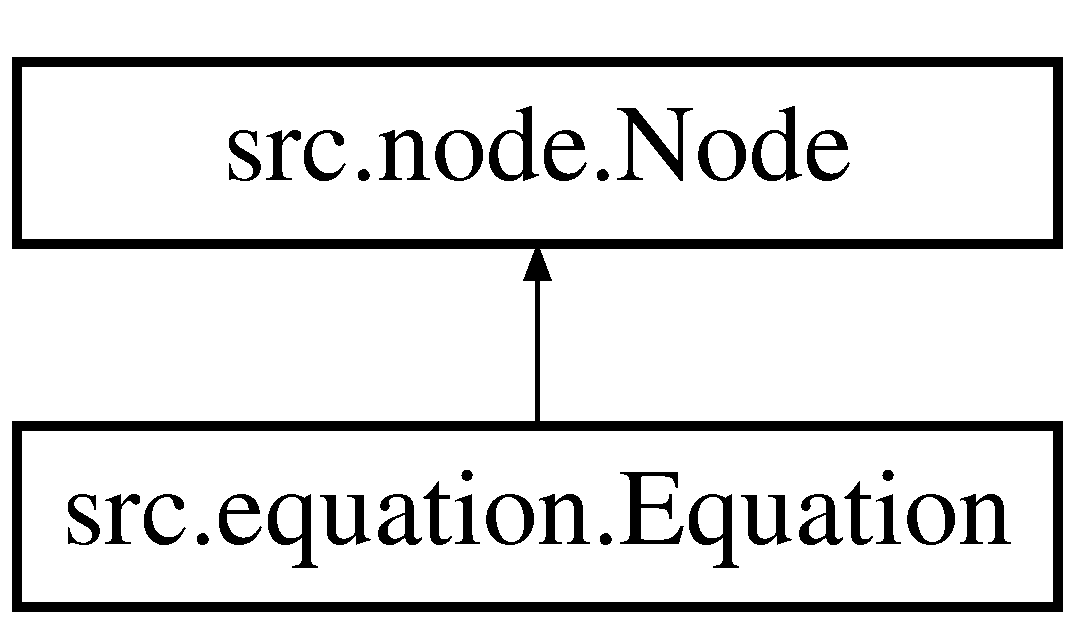
\includegraphics[height=2.000000cm]{classsrc_1_1equation_1_1Equation}
\end{center}
\end{figure}
\subsection*{Public Member Functions}
\begin{DoxyCompactItemize}
\item 
\mbox{\Hypertarget{classsrc_1_1equation_1_1Equation_a4bf4ab4548bc637d3c47c88f41c67ba2}\label{classsrc_1_1equation_1_1Equation_a4bf4ab4548bc637d3c47c88f41c67ba2}} 
def {\bfseries \+\_\+\+\_\+init\+\_\+\+\_\+} (self, left, right)
\item 
\mbox{\Hypertarget{classsrc_1_1equation_1_1Equation_a689f6c4e232d60aa2fba44b46f46dcc3}\label{classsrc_1_1equation_1_1Equation_a689f6c4e232d60aa2fba44b46f46dcc3}} 
def {\bfseries find\+\_\+parts} (self)
\end{DoxyCompactItemize}
\subsection*{Public Attributes}
\begin{DoxyCompactItemize}
\item 
\mbox{\Hypertarget{classsrc_1_1equation_1_1Equation_a8f458f87548078811f4d21c706f88d0e}\label{classsrc_1_1equation_1_1Equation_a8f458f87548078811f4d21c706f88d0e}} 
{\bfseries node}
\item 
\mbox{\Hypertarget{classsrc_1_1equation_1_1Equation_a38186427bf6e964532dbde7f3f8519be}\label{classsrc_1_1equation_1_1Equation_a38186427bf6e964532dbde7f3f8519be}} 
{\bfseries unknowns}
\item 
\mbox{\Hypertarget{classsrc_1_1equation_1_1Equation_a24288eb132057dc0dc2bf547f5ab32b3}\label{classsrc_1_1equation_1_1Equation_a24288eb132057dc0dc2bf547f5ab32b3}} 
{\bfseries constant}
\item 
\mbox{\Hypertarget{classsrc_1_1equation_1_1Equation_a177b39b70a07e6cec9b1a36124e76fe5}\label{classsrc_1_1equation_1_1Equation_a177b39b70a07e6cec9b1a36124e76fe5}} 
{\bfseries number\+\_\+unknowns}
\item 
\mbox{\Hypertarget{classsrc_1_1equation_1_1Equation_adee9115ac8781878f65753bc132c42d7}\label{classsrc_1_1equation_1_1Equation_adee9115ac8781878f65753bc132c42d7}} 
{\bfseries unknown}
\item 
\mbox{\Hypertarget{classsrc_1_1equation_1_1Equation_aa1f7d40ad0e5194c7ab4dad1627b5903}\label{classsrc_1_1equation_1_1Equation_aa1f7d40ad0e5194c7ab4dad1627b5903}} 
{\bfseries grade}
\item 
\mbox{\Hypertarget{classsrc_1_1equation_1_1Equation_a2d8654923394a223fbcd206b4ab208f6}\label{classsrc_1_1equation_1_1Equation_a2d8654923394a223fbcd206b4ab208f6}} 
{\bfseries exponents}
\end{DoxyCompactItemize}


The documentation for this class was generated from the following file\+:\begin{DoxyCompactItemize}
\item 
src/equation.\+py\end{DoxyCompactItemize}

\hypertarget{classsrc_1_1operators_1_1HomogenOperator}{}\section{src.\+operators.\+Homogen\+Operator Class Reference}
\label{classsrc_1_1operators_1_1HomogenOperator}\index{src.\+operators.\+Homogen\+Operator@{src.\+operators.\+Homogen\+Operator}}
Inheritance diagram for src.\+operators.\+Homogen\+Operator\+:\begin{figure}[H]
\begin{center}
\leavevmode
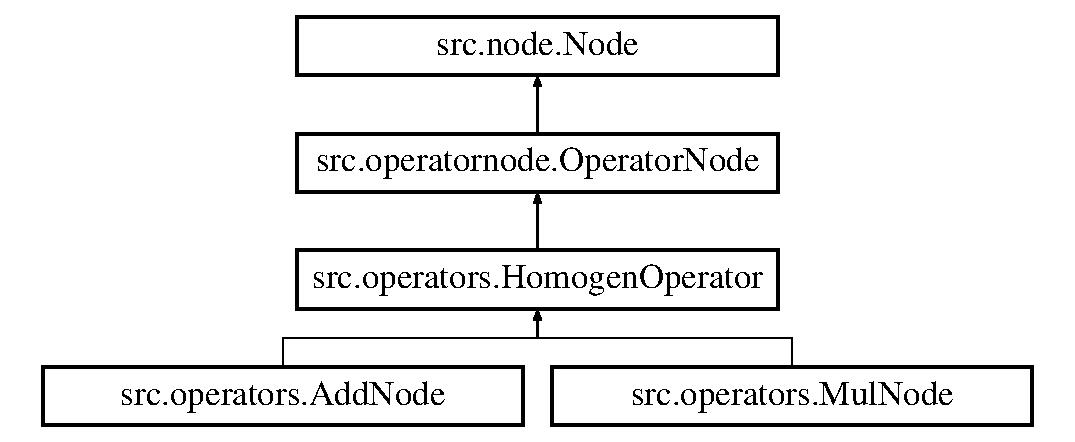
\includegraphics[height=4.000000cm]{classsrc_1_1operators_1_1HomogenOperator}
\end{center}
\end{figure}
\subsection*{Public Member Functions}
\begin{DoxyCompactItemize}
\item 
\mbox{\Hypertarget{classsrc_1_1operators_1_1HomogenOperator_a16a31d31bd2cf3587179af6a9686c827}\label{classsrc_1_1operators_1_1HomogenOperator_a16a31d31bd2cf3587179af6a9686c827}} 
def {\bfseries \+\_\+\+\_\+init\+\_\+\+\_\+} (self, symbol, terms)
\item 
\mbox{\Hypertarget{classsrc_1_1operators_1_1HomogenOperator_a89cdd651ea377c8b8460f4afd1f11c43}\label{classsrc_1_1operators_1_1HomogenOperator_a89cdd651ea377c8b8460f4afd1f11c43}} 
def {\bfseries \+\_\+\+\_\+hash\+\_\+\+\_\+} (self)
\item 
\mbox{\Hypertarget{classsrc_1_1operators_1_1HomogenOperator_a35d32a7d4d52e7fba6720ba2b70cd3e0}\label{classsrc_1_1operators_1_1HomogenOperator_a35d32a7d4d52e7fba6720ba2b70cd3e0}} 
def {\bfseries formatted} (self)
\item 
\mbox{\Hypertarget{classsrc_1_1operators_1_1HomogenOperator_a0bd55b6ad580d42bd11300ac43733d53}\label{classsrc_1_1operators_1_1HomogenOperator_a0bd55b6ad580d42bd11300ac43733d53}} 
def {\bfseries merge\+\_\+in} (self, nodes)
\item 
\mbox{\Hypertarget{classsrc_1_1operators_1_1HomogenOperator_a2bb7c65aa50bcce6c4e70a7e0a9efff4}\label{classsrc_1_1operators_1_1HomogenOperator_a2bb7c65aa50bcce6c4e70a7e0a9efff4}} 
def {\bfseries merge\+\_\+two} (self, term, node)
\item 
\mbox{\Hypertarget{classsrc_1_1operators_1_1HomogenOperator_addaed624b21630ff5c19bddfafab1d7b}\label{classsrc_1_1operators_1_1HomogenOperator_addaed624b21630ff5c19bddfafab1d7b}} 
def {\bfseries get\+\_\+children} (self)
\end{DoxyCompactItemize}
\subsection*{Public Attributes}
\begin{DoxyCompactItemize}
\item 
\mbox{\Hypertarget{classsrc_1_1operators_1_1HomogenOperator_a3bb9a878e36a36cc1131c809ddc4cb0d}\label{classsrc_1_1operators_1_1HomogenOperator_a3bb9a878e36a36cc1131c809ddc4cb0d}} 
{\bfseries terms}
\item 
\mbox{\Hypertarget{classsrc_1_1operators_1_1HomogenOperator_a86b81332395e1f3663fb1dd04a8e5640}\label{classsrc_1_1operators_1_1HomogenOperator_a86b81332395e1f3663fb1dd04a8e5640}} 
{\bfseries symbol}
\end{DoxyCompactItemize}


The documentation for this class was generated from the following file\+:\begin{DoxyCompactItemize}
\item 
src/operators.\+py\end{DoxyCompactItemize}

\hypertarget{classsrc_1_1intnode_1_1IntNode}{}\section{src.\+intnode.\+Int\+Node Class Reference}
\label{classsrc_1_1intnode_1_1IntNode}\index{src.\+intnode.\+Int\+Node@{src.\+intnode.\+Int\+Node}}
Inheritance diagram for src.\+intnode.\+Int\+Node\+:\begin{figure}[H]
\begin{center}
\leavevmode
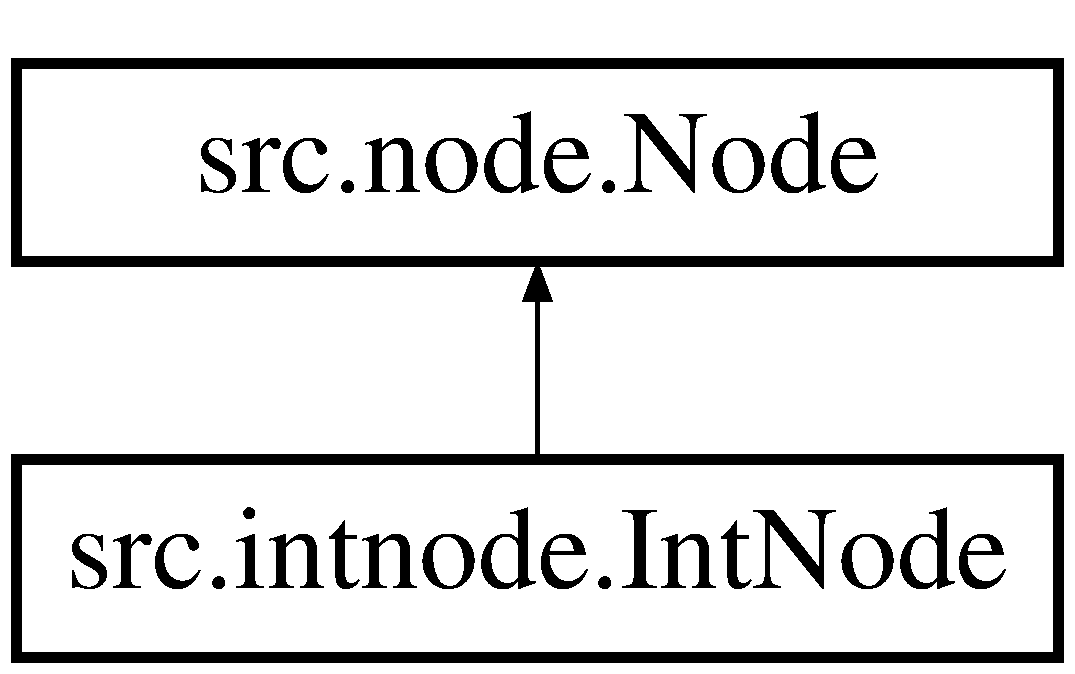
\includegraphics[height=2.000000cm]{classsrc_1_1intnode_1_1IntNode}
\end{center}
\end{figure}
\subsection*{Public Member Functions}
\begin{DoxyCompactItemize}
\item 
\mbox{\Hypertarget{classsrc_1_1intnode_1_1IntNode_afa6814e2e067d1344f4d523c2d1d03ec}\label{classsrc_1_1intnode_1_1IntNode_afa6814e2e067d1344f4d523c2d1d03ec}} 
def {\bfseries \+\_\+\+\_\+init\+\_\+\+\_\+} (self, n)
\item 
\mbox{\Hypertarget{classsrc_1_1intnode_1_1IntNode_a2a0e6ad7ca6d6789e73fc7926f78198d}\label{classsrc_1_1intnode_1_1IntNode_a2a0e6ad7ca6d6789e73fc7926f78198d}} 
def {\bfseries \+\_\+\+\_\+hash\+\_\+\+\_\+} (self)
\item 
\mbox{\Hypertarget{classsrc_1_1intnode_1_1IntNode_a3c3758fa9303abfbe9ce07ea4299ef47}\label{classsrc_1_1intnode_1_1IntNode_a3c3758fa9303abfbe9ce07ea4299ef47}} 
def {\bfseries eval} (self)
\item 
\mbox{\Hypertarget{classsrc_1_1intnode_1_1IntNode_aa0626a04aaf98541d2265fed11926ba5}\label{classsrc_1_1intnode_1_1IntNode_aa0626a04aaf98541d2265fed11926ba5}} 
def {\bfseries simplifyed} (self)
\item 
\mbox{\Hypertarget{classsrc_1_1intnode_1_1IntNode_ac062b5a24b3b320628feeba54e2b4d14}\label{classsrc_1_1intnode_1_1IntNode_ac062b5a24b3b320628feeba54e2b4d14}} 
def {\bfseries formatted} (self)
\item 
\mbox{\Hypertarget{classsrc_1_1intnode_1_1IntNode_ac31637612bd5ac0321833af46ec4a284}\label{classsrc_1_1intnode_1_1IntNode_ac31637612bd5ac0321833af46ec4a284}} 
def {\bfseries contains} (self, value)
\item 
\mbox{\Hypertarget{classsrc_1_1intnode_1_1IntNode_aa4a42ff77fb10c1775b860a16c6c1a06}\label{classsrc_1_1intnode_1_1IntNode_aa4a42ff77fb10c1775b860a16c6c1a06}} 
def {\bfseries get\+\_\+children} (self)
\item 
\mbox{\Hypertarget{classsrc_1_1intnode_1_1IntNode_af79b733bb531756ef27e27fcc0300fd6}\label{classsrc_1_1intnode_1_1IntNode_af79b733bb531756ef27e27fcc0300fd6}} 
def {\bfseries contains\+\_\+unknown} (self)
\item 
\mbox{\Hypertarget{classsrc_1_1intnode_1_1IntNode_aa816f0f1c1c8df30e9e9615572b700b9}\label{classsrc_1_1intnode_1_1IntNode_aa816f0f1c1c8df30e9e9615572b700b9}} 
def {\bfseries latex} (self)
\end{DoxyCompactItemize}
\subsection*{Public Attributes}
\begin{DoxyCompactItemize}
\item 
\mbox{\Hypertarget{classsrc_1_1intnode_1_1IntNode_a976ab1aa8188e41167af1b0a76050352}\label{classsrc_1_1intnode_1_1IntNode_a976ab1aa8188e41167af1b0a76050352}} 
{\bfseries n}
\end{DoxyCompactItemize}


The documentation for this class was generated from the following file\+:\begin{DoxyCompactItemize}
\item 
src/intnode.\+py\end{DoxyCompactItemize}

\hypertarget{classsrc_1_1solvers_1_1Method}{}\section{src.\+solvers.\+Method Class Reference}
\label{classsrc_1_1solvers_1_1Method}\index{src.\+solvers.\+Method@{src.\+solvers.\+Method}}
\subsection*{Public Member Functions}
\begin{DoxyCompactItemize}
\item 
\mbox{\Hypertarget{classsrc_1_1solvers_1_1Method_a6c478eb58abd4ef7915f98ea0a127300}\label{classsrc_1_1solvers_1_1Method_a6c478eb58abd4ef7915f98ea0a127300}} 
def {\bfseries \+\_\+\+\_\+init\+\_\+\+\_\+} (self, function, grade=None)
\item 
\mbox{\Hypertarget{classsrc_1_1solvers_1_1Method_a945b4fda3e0e9376f49c90bdd7e2cc93}\label{classsrc_1_1solvers_1_1Method_a945b4fda3e0e9376f49c90bdd7e2cc93}} 
def {\bfseries matches} (self, grade)
\end{DoxyCompactItemize}
\subsection*{Public Attributes}
\begin{DoxyCompactItemize}
\item 
\mbox{\Hypertarget{classsrc_1_1solvers_1_1Method_a341727ead36b9976f302c5a598398d95}\label{classsrc_1_1solvers_1_1Method_a341727ead36b9976f302c5a598398d95}} 
{\bfseries grade}
\item 
\mbox{\Hypertarget{classsrc_1_1solvers_1_1Method_a786f42fa2ac57ac0c1a99b173ffd1a84}\label{classsrc_1_1solvers_1_1Method_a786f42fa2ac57ac0c1a99b173ffd1a84}} 
{\bfseries function}
\end{DoxyCompactItemize}


The documentation for this class was generated from the following file\+:\begin{DoxyCompactItemize}
\item 
src/solvers.\+py\end{DoxyCompactItemize}

\hypertarget{classsrc_1_1operators_1_1MulNode}{}\section{src.\+operators.\+Mul\+Node Class Reference}
\label{classsrc_1_1operators_1_1MulNode}\index{src.\+operators.\+Mul\+Node@{src.\+operators.\+Mul\+Node}}
Inheritance diagram for src.\+operators.\+Mul\+Node\+:\begin{figure}[H]
\begin{center}
\leavevmode
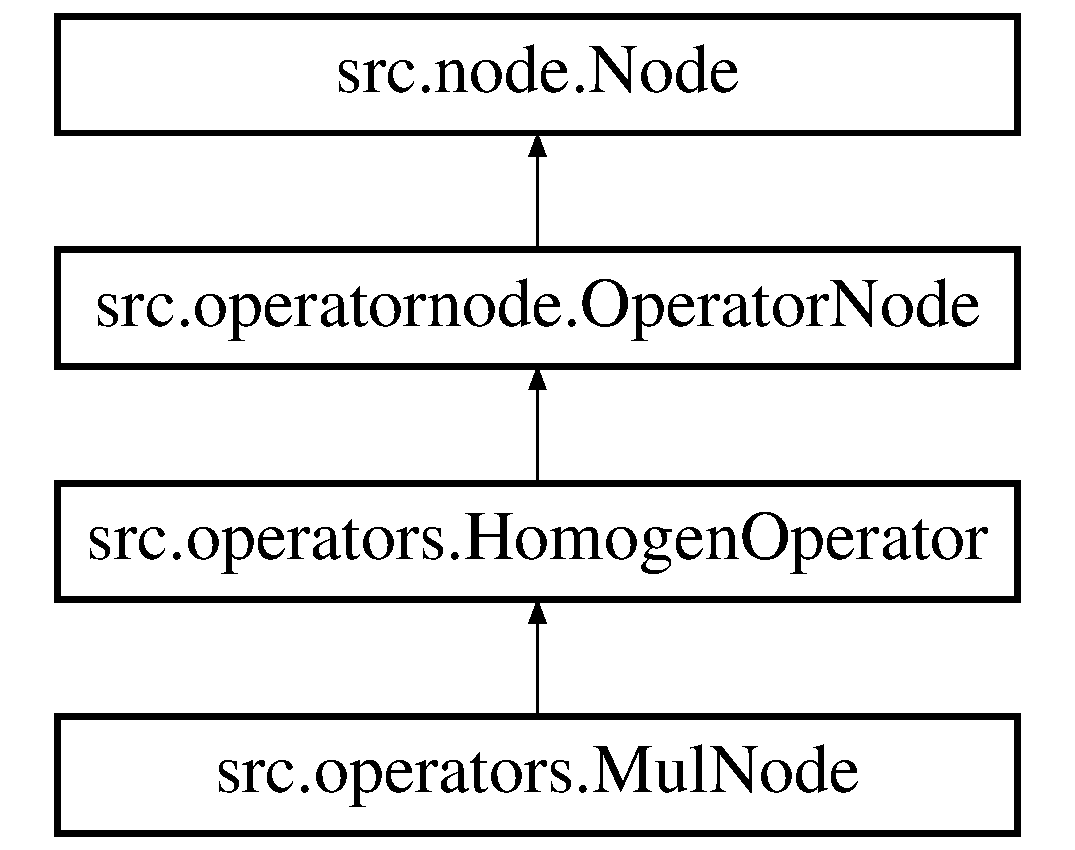
\includegraphics[height=4.000000cm]{classsrc_1_1operators_1_1MulNode}
\end{center}
\end{figure}
\subsection*{Public Member Functions}
\begin{DoxyCompactItemize}
\item 
\mbox{\Hypertarget{classsrc_1_1operators_1_1MulNode_a1ffc386bdbe2f295ce738a52bb518c02}\label{classsrc_1_1operators_1_1MulNode_a1ffc386bdbe2f295ce738a52bb518c02}} 
def {\bfseries \+\_\+\+\_\+init\+\_\+\+\_\+} (self, terms)
\item 
\mbox{\Hypertarget{classsrc_1_1operators_1_1MulNode_a0f9630eb9a8431236eff6c33744e1ed2}\label{classsrc_1_1operators_1_1MulNode_a0f9630eb9a8431236eff6c33744e1ed2}} 
def {\bfseries eval} (self)
\item 
\mbox{\Hypertarget{classsrc_1_1operators_1_1MulNode_ad8b67ebaeb713e18348a86495496b509}\label{classsrc_1_1operators_1_1MulNode_ad8b67ebaeb713e18348a86495496b509}} 
def {\bfseries merge\+\_\+two} (self, term, node)
\item 
\mbox{\Hypertarget{classsrc_1_1operators_1_1MulNode_aa5438e735309074305027f6aed89ae3a}\label{classsrc_1_1operators_1_1MulNode_aa5438e735309074305027f6aed89ae3a}} 
def {\bfseries simplifyed} (self)
\item 
\mbox{\Hypertarget{classsrc_1_1operators_1_1MulNode_ab7b8c4c9c2af8aa24217ea7ae3534866}\label{classsrc_1_1operators_1_1MulNode_ab7b8c4c9c2af8aa24217ea7ae3534866}} 
def {\bfseries latex} (self)
\end{DoxyCompactItemize}
\subsection*{Additional Inherited Members}


The documentation for this class was generated from the following file\+:\begin{DoxyCompactItemize}
\item 
src/operators.\+py\end{DoxyCompactItemize}

\hypertarget{classsrc_1_1node_1_1Node}{}\section{src.\+node.\+Node Class Reference}
\label{classsrc_1_1node_1_1Node}\index{src.\+node.\+Node@{src.\+node.\+Node}}
Inheritance diagram for src.\+node.\+Node\+:\begin{figure}[H]
\begin{center}
\leavevmode
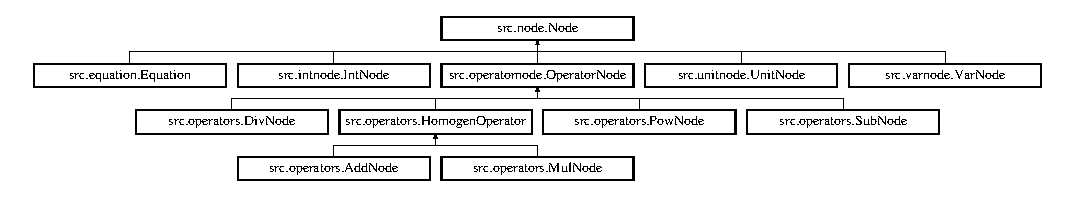
\includegraphics[height=2.196079cm]{classsrc_1_1node_1_1Node}
\end{center}
\end{figure}
\subsection*{Public Member Functions}
\begin{DoxyCompactItemize}
\item 
\mbox{\Hypertarget{classsrc_1_1node_1_1Node_a933de5ee7e799d2538da89c0bdb1f67c}\label{classsrc_1_1node_1_1Node_a933de5ee7e799d2538da89c0bdb1f67c}} 
def {\bfseries \+\_\+\+\_\+init\+\_\+\+\_\+} (self)
\item 
\mbox{\Hypertarget{classsrc_1_1node_1_1Node_a55e38c6599bc88e7488c9afbb7eaa100}\label{classsrc_1_1node_1_1Node_a55e38c6599bc88e7488c9afbb7eaa100}} 
def {\bfseries \+\_\+\+\_\+add\+\_\+\+\_\+} (self, other)
\item 
\mbox{\Hypertarget{classsrc_1_1node_1_1Node_aee34af65ac3e10545f3615b2239ba8a6}\label{classsrc_1_1node_1_1Node_aee34af65ac3e10545f3615b2239ba8a6}} 
def {\bfseries \+\_\+\+\_\+sub\+\_\+\+\_\+} (self, other)
\item 
\mbox{\Hypertarget{classsrc_1_1node_1_1Node_a93320354a3b0a110a70849690e38c8ae}\label{classsrc_1_1node_1_1Node_a93320354a3b0a110a70849690e38c8ae}} 
def {\bfseries \+\_\+\+\_\+mul\+\_\+\+\_\+} (self, other)
\item 
\mbox{\Hypertarget{classsrc_1_1node_1_1Node_a9e54c9ae0209f7810fd476b7858a9f96}\label{classsrc_1_1node_1_1Node_a9e54c9ae0209f7810fd476b7858a9f96}} 
def {\bfseries \+\_\+\+\_\+truediv\+\_\+\+\_\+} (self, other)
\item 
\mbox{\Hypertarget{classsrc_1_1node_1_1Node_ac9c4ad81dff8293294cb2595d26f7e5c}\label{classsrc_1_1node_1_1Node_ac9c4ad81dff8293294cb2595d26f7e5c}} 
def {\bfseries \+\_\+\+\_\+pow\+\_\+\+\_\+} (self, other)
\item 
\mbox{\Hypertarget{classsrc_1_1node_1_1Node_ad67a6d5e78b7221fb36d43b1e32f8abb}\label{classsrc_1_1node_1_1Node_ad67a6d5e78b7221fb36d43b1e32f8abb}} 
def {\bfseries \+\_\+\+\_\+hash\+\_\+\+\_\+} (self)
\item 
\mbox{\Hypertarget{classsrc_1_1node_1_1Node_a4597de2c85ad4dac161259e55d8effb3}\label{classsrc_1_1node_1_1Node_a4597de2c85ad4dac161259e55d8effb3}} 
def {\bfseries \+\_\+\+\_\+str\+\_\+\+\_\+} (self)
\item 
\mbox{\Hypertarget{classsrc_1_1node_1_1Node_a552690bac0476fac1be3dbeb93a8f358}\label{classsrc_1_1node_1_1Node_a552690bac0476fac1be3dbeb93a8f358}} 
def {\bfseries \+\_\+\+\_\+format\+\_\+\+\_\+} (self, format\+\_\+spec)
\item 
def \mbox{\hyperlink{classsrc_1_1node_1_1Node_a756ae69f487fdee0a12e5f462d805c3e}{get\+\_\+children}} (self)
\item 
def \mbox{\hyperlink{classsrc_1_1node_1_1Node_ab8922015ef650c8c490bd57bb247cdb3}{formatted}} (self)
\item 
\mbox{\Hypertarget{classsrc_1_1node_1_1Node_ad67a6d5e78b7221fb36d43b1e32f8abb}\label{classsrc_1_1node_1_1Node_ad67a6d5e78b7221fb36d43b1e32f8abb}} 
def {\bfseries \+\_\+\+\_\+hash\+\_\+\+\_\+} (self)
\item 
def \mbox{\hyperlink{classsrc_1_1node_1_1Node_af95402801ea0022078ff5adb2f21bcf4}{eval}} (self)
\item 
def \mbox{\hyperlink{classsrc_1_1node_1_1Node_a78a051abb54de2b49a557c780d53c05b}{simplifyed}} (self)
\item 
\mbox{\Hypertarget{classsrc_1_1node_1_1Node_ac2692decc5f1f31c630b33032ccda24d}\label{classsrc_1_1node_1_1Node_ac2692decc5f1f31c630b33032ccda24d}} 
def {\bfseries simplify} (self)
\item 
def \mbox{\hyperlink{classsrc_1_1node_1_1Node_a96e5e408dd0bcca509adb992b3896010}{latex}} (self)
\item 
def \mbox{\hyperlink{classsrc_1_1node_1_1Node_a08d924ae213016952cc4a520a961d945}{contains\+\_\+unknowns}} (self)
\item 
def \mbox{\hyperlink{classsrc_1_1node_1_1Node_aca2d7597667efc35f903fd455cb1c5fb}{contains}} (self, value)
\end{DoxyCompactItemize}


\subsection{Detailed Description}
\begin{DoxyVerb}Base class for all nodes. Not meant to be used to be directly used only extended
\end{DoxyVerb}
 

\subsection{Member Function Documentation}
\mbox{\Hypertarget{classsrc_1_1node_1_1Node_aca2d7597667efc35f903fd455cb1c5fb}\label{classsrc_1_1node_1_1Node_aca2d7597667efc35f903fd455cb1c5fb}} 
\index{src\+::node\+::\+Node@{src\+::node\+::\+Node}!contains@{contains}}
\index{contains@{contains}!src\+::node\+::\+Node@{src\+::node\+::\+Node}}
\subsubsection{\texorpdfstring{contains()}{contains()}}
{\footnotesize\ttfamily def src.\+node.\+Node.\+contains (\begin{DoxyParamCaption}\item[{}]{self,  }\item[{}]{value }\end{DoxyParamCaption})}

\begin{DoxyVerb}Uses the get_children() method to recursively check for a node. Override on nodes without children.
\end{DoxyVerb}
 \mbox{\Hypertarget{classsrc_1_1node_1_1Node_a08d924ae213016952cc4a520a961d945}\label{classsrc_1_1node_1_1Node_a08d924ae213016952cc4a520a961d945}} 
\index{src\+::node\+::\+Node@{src\+::node\+::\+Node}!contains\+\_\+unknowns@{contains\+\_\+unknowns}}
\index{contains\+\_\+unknowns@{contains\+\_\+unknowns}!src\+::node\+::\+Node@{src\+::node\+::\+Node}}
\subsubsection{\texorpdfstring{contains\+\_\+unknowns()}{contains\_unknowns()}}
{\footnotesize\ttfamily def src.\+node.\+Node.\+contains\+\_\+unknowns (\begin{DoxyParamCaption}\item[{}]{self }\end{DoxyParamCaption})}

\begin{DoxyVerb}Uses the get_children method to recursively check for unknowns. Override on nodes without children.
\end{DoxyVerb}
 \mbox{\Hypertarget{classsrc_1_1node_1_1Node_af95402801ea0022078ff5adb2f21bcf4}\label{classsrc_1_1node_1_1Node_af95402801ea0022078ff5adb2f21bcf4}} 
\index{src\+::node\+::\+Node@{src\+::node\+::\+Node}!eval@{eval}}
\index{eval@{eval}!src\+::node\+::\+Node@{src\+::node\+::\+Node}}
\subsubsection{\texorpdfstring{eval()}{eval()}}
{\footnotesize\ttfamily def src.\+node.\+Node.\+eval (\begin{DoxyParamCaption}\item[{}]{self }\end{DoxyParamCaption})}

\begin{DoxyVerb}Calculates the approxemate value of the node.
\end{DoxyVerb}
 \mbox{\Hypertarget{classsrc_1_1node_1_1Node_ab8922015ef650c8c490bd57bb247cdb3}\label{classsrc_1_1node_1_1Node_ab8922015ef650c8c490bd57bb247cdb3}} 
\index{src\+::node\+::\+Node@{src\+::node\+::\+Node}!formatted@{formatted}}
\index{formatted@{formatted}!src\+::node\+::\+Node@{src\+::node\+::\+Node}}
\subsubsection{\texorpdfstring{formatted()}{formatted()}}
{\footnotesize\ttfamily def src.\+node.\+Node.\+formatted (\begin{DoxyParamCaption}\item[{}]{self }\end{DoxyParamCaption})}

\begin{DoxyVerb}Return a text representation of the node
\end{DoxyVerb}
 \mbox{\Hypertarget{classsrc_1_1node_1_1Node_a756ae69f487fdee0a12e5f462d805c3e}\label{classsrc_1_1node_1_1Node_a756ae69f487fdee0a12e5f462d805c3e}} 
\index{src\+::node\+::\+Node@{src\+::node\+::\+Node}!get\+\_\+children@{get\+\_\+children}}
\index{get\+\_\+children@{get\+\_\+children}!src\+::node\+::\+Node@{src\+::node\+::\+Node}}
\subsubsection{\texorpdfstring{get\+\_\+children()}{get\_children()}}
{\footnotesize\ttfamily def src.\+node.\+Node.\+get\+\_\+children (\begin{DoxyParamCaption}\item[{}]{self }\end{DoxyParamCaption})}

\begin{DoxyVerb}Returns The children of a node returns node if no children.
\end{DoxyVerb}
 \mbox{\Hypertarget{classsrc_1_1node_1_1Node_a96e5e408dd0bcca509adb992b3896010}\label{classsrc_1_1node_1_1Node_a96e5e408dd0bcca509adb992b3896010}} 
\index{src\+::node\+::\+Node@{src\+::node\+::\+Node}!latex@{latex}}
\index{latex@{latex}!src\+::node\+::\+Node@{src\+::node\+::\+Node}}
\subsubsection{\texorpdfstring{latex()}{latex()}}
{\footnotesize\ttfamily def src.\+node.\+Node.\+latex (\begin{DoxyParamCaption}\item[{}]{self }\end{DoxyParamCaption})}

\begin{DoxyVerb}Return latex for the node.
\end{DoxyVerb}
 \mbox{\Hypertarget{classsrc_1_1node_1_1Node_a78a051abb54de2b49a557c780d53c05b}\label{classsrc_1_1node_1_1Node_a78a051abb54de2b49a557c780d53c05b}} 
\index{src\+::node\+::\+Node@{src\+::node\+::\+Node}!simplifyed@{simplifyed}}
\index{simplifyed@{simplifyed}!src\+::node\+::\+Node@{src\+::node\+::\+Node}}
\subsubsection{\texorpdfstring{simplifyed()}{simplifyed()}}
{\footnotesize\ttfamily def src.\+node.\+Node.\+simplifyed (\begin{DoxyParamCaption}\item[{}]{self }\end{DoxyParamCaption})}

\begin{DoxyVerb}Return a simplifyed clone of the node.
\end{DoxyVerb}
 

The documentation for this class was generated from the following file\+:\begin{DoxyCompactItemize}
\item 
src/node.\+py\end{DoxyCompactItemize}

\hypertarget{classsrc_1_1operator__gen_1_1Operator}{}\section{src.\+operator\+\_\+gen.\+Operator Class Reference}
\label{classsrc_1_1operator__gen_1_1Operator}\index{src.\+operator\+\_\+gen.\+Operator@{src.\+operator\+\_\+gen.\+Operator}}
\subsection*{Public Member Functions}
\begin{DoxyCompactItemize}
\item 
\mbox{\Hypertarget{classsrc_1_1operator__gen_1_1Operator_a4b22d090915d41d0814bb5b9662632bb}\label{classsrc_1_1operator__gen_1_1Operator_a4b22d090915d41d0814bb5b9662632bb}} 
def {\bfseries \+\_\+\+\_\+init\+\_\+\+\_\+} (self, name, operator, multi=False)
\item 
\mbox{\Hypertarget{classsrc_1_1operator__gen_1_1Operator_a159119b5a1c6e8dccc1d7e2ef71ac632}\label{classsrc_1_1operator__gen_1_1Operator_a159119b5a1c6e8dccc1d7e2ef71ac632}} 
def {\bfseries gen} (self)
\end{DoxyCompactItemize}
\subsection*{Public Attributes}
\begin{DoxyCompactItemize}
\item 
\mbox{\Hypertarget{classsrc_1_1operator__gen_1_1Operator_a1655cab034b2c4df42b0b0d1db642138}\label{classsrc_1_1operator__gen_1_1Operator_a1655cab034b2c4df42b0b0d1db642138}} 
{\bfseries name}
\item 
\mbox{\Hypertarget{classsrc_1_1operator__gen_1_1Operator_a1e578bc37692ea3ca86404adf874a872}\label{classsrc_1_1operator__gen_1_1Operator_a1e578bc37692ea3ca86404adf874a872}} 
{\bfseries operator}
\end{DoxyCompactItemize}
\subsection*{Static Public Attributes}
\begin{DoxyCompactItemize}
\item 
\mbox{\Hypertarget{classsrc_1_1operator__gen_1_1Operator_afb1f4aa4409dd8a25b2f0f560aafae86}\label{classsrc_1_1operator__gen_1_1Operator_afb1f4aa4409dd8a25b2f0f560aafae86}} 
{\bfseries multi}
\end{DoxyCompactItemize}


The documentation for this class was generated from the following file\+:\begin{DoxyCompactItemize}
\item 
src/operator\+\_\+gen.\+py\end{DoxyCompactItemize}

\hypertarget{classsrc_1_1operatornode_1_1OperatorNode}{}\section{src.\+operatornode.\+Operator\+Node Class Reference}
\label{classsrc_1_1operatornode_1_1OperatorNode}\index{src.\+operatornode.\+Operator\+Node@{src.\+operatornode.\+Operator\+Node}}
Inheritance diagram for src.\+operatornode.\+Operator\+Node\+:\begin{figure}[H]
\begin{center}
\leavevmode
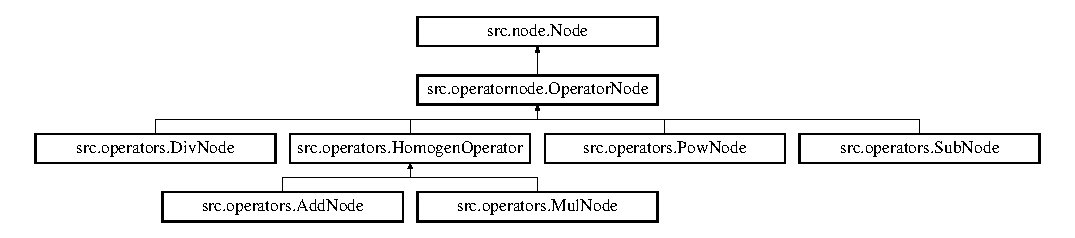
\includegraphics[height=2.745098cm]{classsrc_1_1operatornode_1_1OperatorNode}
\end{center}
\end{figure}
\subsection*{Public Member Functions}
\begin{DoxyCompactItemize}
\item 
\mbox{\Hypertarget{classsrc_1_1operatornode_1_1OperatorNode_a8a52d701bbf1460c52777f16c510f184}\label{classsrc_1_1operatornode_1_1OperatorNode_a8a52d701bbf1460c52777f16c510f184}} 
def {\bfseries \+\_\+\+\_\+init\+\_\+\+\_\+} (self)
\end{DoxyCompactItemize}


The documentation for this class was generated from the following file\+:\begin{DoxyCompactItemize}
\item 
src/operatornode.\+py\end{DoxyCompactItemize}

\hypertarget{classsrc_1_1operators_1_1PowNode}{}\section{src.\+operators.\+Pow\+Node Class Reference}
\label{classsrc_1_1operators_1_1PowNode}\index{src.\+operators.\+Pow\+Node@{src.\+operators.\+Pow\+Node}}
Inheritance diagram for src.\+operators.\+Pow\+Node\+:\begin{figure}[H]
\begin{center}
\leavevmode
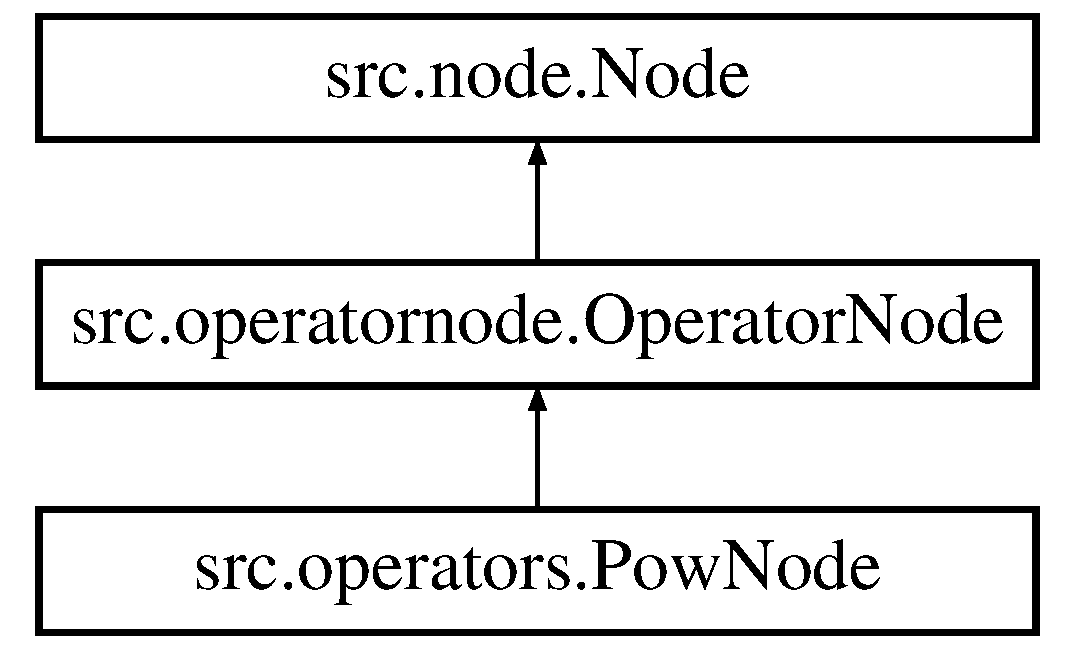
\includegraphics[height=3.000000cm]{classsrc_1_1operators_1_1PowNode}
\end{center}
\end{figure}
\subsection*{Public Member Functions}
\begin{DoxyCompactItemize}
\item 
\mbox{\Hypertarget{classsrc_1_1operators_1_1PowNode_a5fa7636ca29e14313d3d4fbfda132a44}\label{classsrc_1_1operators_1_1PowNode_a5fa7636ca29e14313d3d4fbfda132a44}} 
def {\bfseries \+\_\+\+\_\+init\+\_\+\+\_\+} (self, left, right)
\item 
\mbox{\Hypertarget{classsrc_1_1operators_1_1PowNode_a69b1f29b606f3ed9f5fb6e4acbf299d7}\label{classsrc_1_1operators_1_1PowNode_a69b1f29b606f3ed9f5fb6e4acbf299d7}} 
def {\bfseries \+\_\+\+\_\+hash\+\_\+\+\_\+} (self)
\item 
\mbox{\Hypertarget{classsrc_1_1operators_1_1PowNode_a63017687d2d16840023e42dc22b8fc2b}\label{classsrc_1_1operators_1_1PowNode_a63017687d2d16840023e42dc22b8fc2b}} 
def {\bfseries eval} (self)
\item 
\mbox{\Hypertarget{classsrc_1_1operators_1_1PowNode_a45d0e4cb2217f175e3c31c750c129f99}\label{classsrc_1_1operators_1_1PowNode_a45d0e4cb2217f175e3c31c750c129f99}} 
def {\bfseries formatted} (self)
\item 
\mbox{\Hypertarget{classsrc_1_1operators_1_1PowNode_ad9e8821e363fd37762331dc8abb5265a}\label{classsrc_1_1operators_1_1PowNode_ad9e8821e363fd37762331dc8abb5265a}} 
def {\bfseries contains} (self, value)
\item 
\mbox{\Hypertarget{classsrc_1_1operators_1_1PowNode_aec4398a301e3dbf7ec19762fde70521b}\label{classsrc_1_1operators_1_1PowNode_aec4398a301e3dbf7ec19762fde70521b}} 
def {\bfseries simplifyed} (self)
\item 
\mbox{\Hypertarget{classsrc_1_1operators_1_1PowNode_adc7eb91977008ce8bde2d763f7b00c44}\label{classsrc_1_1operators_1_1PowNode_adc7eb91977008ce8bde2d763f7b00c44}} 
def {\bfseries get\+\_\+children} (self)
\item 
\mbox{\Hypertarget{classsrc_1_1operators_1_1PowNode_ad84893a2c9e99d4bbc221399d517d528}\label{classsrc_1_1operators_1_1PowNode_ad84893a2c9e99d4bbc221399d517d528}} 
def {\bfseries latex} (self)
\end{DoxyCompactItemize}
\subsection*{Public Attributes}
\begin{DoxyCompactItemize}
\item 
\mbox{\Hypertarget{classsrc_1_1operators_1_1PowNode_aa0256c2a415b3690514f78ab0ca52ee8}\label{classsrc_1_1operators_1_1PowNode_aa0256c2a415b3690514f78ab0ca52ee8}} 
{\bfseries left}
\item 
\mbox{\Hypertarget{classsrc_1_1operators_1_1PowNode_a12b3318638143cf59a0b50aed6b158e2}\label{classsrc_1_1operators_1_1PowNode_a12b3318638143cf59a0b50aed6b158e2}} 
{\bfseries right}
\end{DoxyCompactItemize}


The documentation for this class was generated from the following file\+:\begin{DoxyCompactItemize}
\item 
src/operators.\+py\end{DoxyCompactItemize}

\hypertarget{classsrc_1_1solvers_1_1Solver}{}\section{src.\+solvers.\+Solver Class Reference}
\label{classsrc_1_1solvers_1_1Solver}\index{src.\+solvers.\+Solver@{src.\+solvers.\+Solver}}
\subsection*{Public Member Functions}
\begin{DoxyCompactItemize}
\item 
\mbox{\Hypertarget{classsrc_1_1solvers_1_1Solver_a5415ed6863748bdccd46e474367577dd}\label{classsrc_1_1solvers_1_1Solver_a5415ed6863748bdccd46e474367577dd}} 
def {\bfseries \+\_\+\+\_\+init\+\_\+\+\_\+} (self)
\item 
\mbox{\Hypertarget{classsrc_1_1solvers_1_1Solver_a76ee174069426212316cbbc8c5440db4}\label{classsrc_1_1solvers_1_1Solver_a76ee174069426212316cbbc8c5440db4}} 
def {\bfseries method} (self, grade=None)
\item 
\mbox{\Hypertarget{classsrc_1_1solvers_1_1Solver_a4bf9eccb3a4ed422f8b74ed43199c023}\label{classsrc_1_1solvers_1_1Solver_a4bf9eccb3a4ed422f8b74ed43199c023}} 
def {\bfseries solve} (self, equation)
\item 
\mbox{\Hypertarget{classsrc_1_1solvers_1_1Solver_a9f92c7a01bf90d6218d528f9fabbfedc}\label{classsrc_1_1solvers_1_1Solver_a9f92c7a01bf90d6218d528f9fabbfedc}} 
def {\bfseries find\+\_\+method} (self, grade=None)
\end{DoxyCompactItemize}
\subsection*{Public Attributes}
\begin{DoxyCompactItemize}
\item 
\mbox{\Hypertarget{classsrc_1_1solvers_1_1Solver_ac6296ecde06930a25d7c13c2fdea98a7}\label{classsrc_1_1solvers_1_1Solver_ac6296ecde06930a25d7c13c2fdea98a7}} 
{\bfseries methods}
\end{DoxyCompactItemize}


The documentation for this class was generated from the following file\+:\begin{DoxyCompactItemize}
\item 
src/solvers.\+py\end{DoxyCompactItemize}

\hypertarget{classsrc_1_1operators_1_1SubNode}{}\section{src.\+operators.\+Sub\+Node Class Reference}
\label{classsrc_1_1operators_1_1SubNode}\index{src.\+operators.\+Sub\+Node@{src.\+operators.\+Sub\+Node}}
Inheritance diagram for src.\+operators.\+Sub\+Node\+:\begin{figure}[H]
\begin{center}
\leavevmode
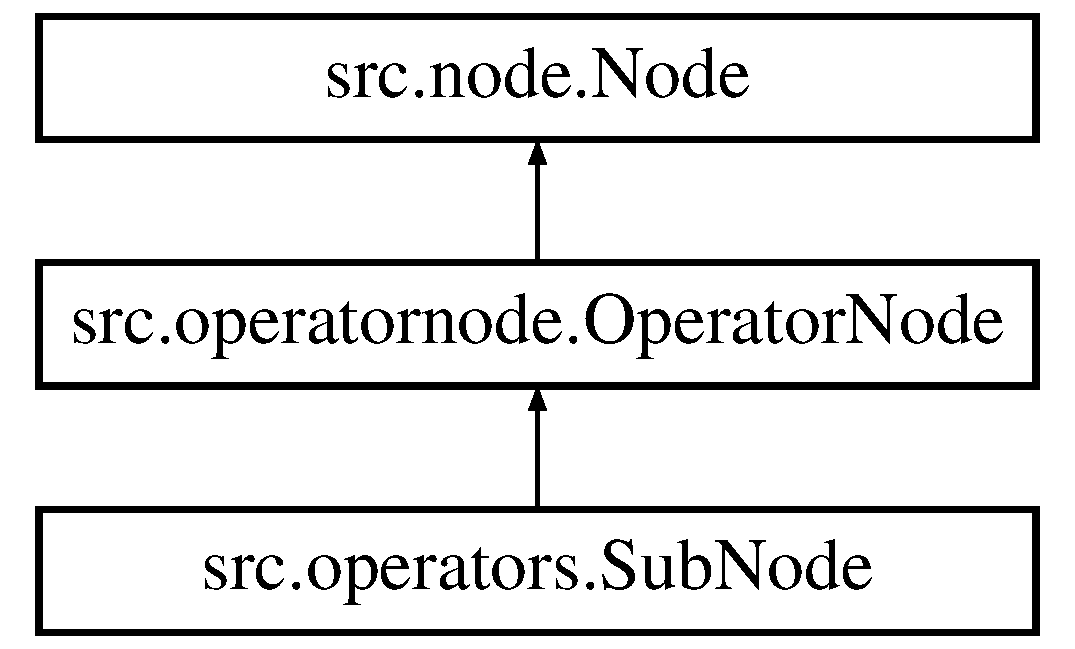
\includegraphics[height=3.000000cm]{classsrc_1_1operators_1_1SubNode}
\end{center}
\end{figure}
\subsection*{Public Member Functions}
\begin{DoxyCompactItemize}
\item 
\mbox{\Hypertarget{classsrc_1_1operators_1_1SubNode_a16fe3afdaf1dd064dea307baf7a224da}\label{classsrc_1_1operators_1_1SubNode_a16fe3afdaf1dd064dea307baf7a224da}} 
def {\bfseries \+\_\+\+\_\+init\+\_\+\+\_\+} (self, left, right)
\item 
\mbox{\Hypertarget{classsrc_1_1operators_1_1SubNode_adc0745a196130d08389b5e92adfa10f5}\label{classsrc_1_1operators_1_1SubNode_adc0745a196130d08389b5e92adfa10f5}} 
def {\bfseries \+\_\+\+\_\+hash\+\_\+\+\_\+} (self)
\item 
\mbox{\Hypertarget{classsrc_1_1operators_1_1SubNode_aa3893c64dbc93a612f7b5cac77c46b9d}\label{classsrc_1_1operators_1_1SubNode_aa3893c64dbc93a612f7b5cac77c46b9d}} 
def {\bfseries eval} (self)
\item 
\mbox{\Hypertarget{classsrc_1_1operators_1_1SubNode_a40115edd84365abcddf4a447d927595c}\label{classsrc_1_1operators_1_1SubNode_a40115edd84365abcddf4a447d927595c}} 
def {\bfseries formatted} (self)
\item 
\mbox{\Hypertarget{classsrc_1_1operators_1_1SubNode_a4ebc919be9178d06b86483ded2cc5804}\label{classsrc_1_1operators_1_1SubNode_a4ebc919be9178d06b86483ded2cc5804}} 
def {\bfseries simplifyed} (self)
\item 
\mbox{\Hypertarget{classsrc_1_1operators_1_1SubNode_af73a5753bd8a68b4f8ea824ecdf01270}\label{classsrc_1_1operators_1_1SubNode_af73a5753bd8a68b4f8ea824ecdf01270}} 
def {\bfseries get\+\_\+children} (self)
\item 
\mbox{\Hypertarget{classsrc_1_1operators_1_1SubNode_ae47f713a60829825fd8c9bc6ca48d0f5}\label{classsrc_1_1operators_1_1SubNode_ae47f713a60829825fd8c9bc6ca48d0f5}} 
def {\bfseries latex} (self)
\end{DoxyCompactItemize}
\subsection*{Public Attributes}
\begin{DoxyCompactItemize}
\item 
\mbox{\Hypertarget{classsrc_1_1operators_1_1SubNode_ade2ff77d06b2233ca6104d4ae137225d}\label{classsrc_1_1operators_1_1SubNode_ade2ff77d06b2233ca6104d4ae137225d}} 
{\bfseries left}
\item 
\mbox{\Hypertarget{classsrc_1_1operators_1_1SubNode_afb1007a19b8e776294f4b58575e4ce54}\label{classsrc_1_1operators_1_1SubNode_afb1007a19b8e776294f4b58575e4ce54}} 
{\bfseries right}
\end{DoxyCompactItemize}


The documentation for this class was generated from the following file\+:\begin{DoxyCompactItemize}
\item 
src/operators.\+py\end{DoxyCompactItemize}

\hypertarget{classsrc_1_1unitnode_1_1UnitNode}{}\section{src.\+unitnode.\+Unit\+Node Class Reference}
\label{classsrc_1_1unitnode_1_1UnitNode}\index{src.\+unitnode.\+Unit\+Node@{src.\+unitnode.\+Unit\+Node}}
Inheritance diagram for src.\+unitnode.\+Unit\+Node\+:\begin{figure}[H]
\begin{center}
\leavevmode
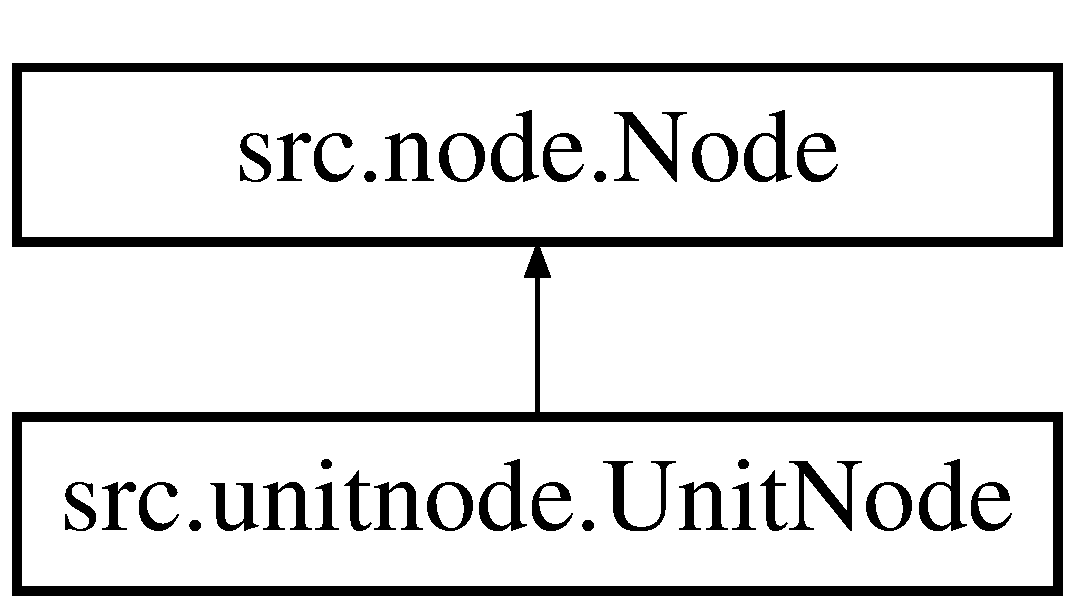
\includegraphics[height=2.000000cm]{classsrc_1_1unitnode_1_1UnitNode}
\end{center}
\end{figure}
\subsection*{Public Member Functions}
\begin{DoxyCompactItemize}
\item 
\mbox{\Hypertarget{classsrc_1_1unitnode_1_1UnitNode_acc72ea269b8094c1b70a4edd1cd4a188}\label{classsrc_1_1unitnode_1_1UnitNode_acc72ea269b8094c1b70a4edd1cd4a188}} 
def {\bfseries \+\_\+\+\_\+init\+\_\+\+\_\+} (self, unit, value)
\item 
\mbox{\Hypertarget{classsrc_1_1unitnode_1_1UnitNode_afcba67317c5fe2f6fada02667591151f}\label{classsrc_1_1unitnode_1_1UnitNode_afcba67317c5fe2f6fada02667591151f}} 
def {\bfseries \+\_\+\+\_\+hash\+\_\+\+\_\+} (self)
\item 
\mbox{\Hypertarget{classsrc_1_1unitnode_1_1UnitNode_af85c10b875266acff02c11d36aba1a92}\label{classsrc_1_1unitnode_1_1UnitNode_af85c10b875266acff02c11d36aba1a92}} 
def {\bfseries simplifyed} (self)
\item 
\mbox{\Hypertarget{classsrc_1_1unitnode_1_1UnitNode_a7b9c4f011f61d4ceeae2172d3631b92d}\label{classsrc_1_1unitnode_1_1UnitNode_a7b9c4f011f61d4ceeae2172d3631b92d}} 
def {\bfseries formatted} (self)
\item 
\mbox{\Hypertarget{classsrc_1_1unitnode_1_1UnitNode_aa707963f0ef8340a3cc09e859eb938e3}\label{classsrc_1_1unitnode_1_1UnitNode_aa707963f0ef8340a3cc09e859eb938e3}} 
def {\bfseries eval} (self)
\item 
\mbox{\Hypertarget{classsrc_1_1unitnode_1_1UnitNode_a2cd4eb0a34ed9d0b1c6fa76975b37033}\label{classsrc_1_1unitnode_1_1UnitNode_a2cd4eb0a34ed9d0b1c6fa76975b37033}} 
def {\bfseries get\+\_\+children} (self)
\item 
\mbox{\Hypertarget{classsrc_1_1unitnode_1_1UnitNode_afbbbbc116b8bbd9497b73e53fb918bbf}\label{classsrc_1_1unitnode_1_1UnitNode_afbbbbc116b8bbd9497b73e53fb918bbf}} 
def {\bfseries latex} (self)
\end{DoxyCompactItemize}
\subsection*{Public Attributes}
\begin{DoxyCompactItemize}
\item 
\mbox{\Hypertarget{classsrc_1_1unitnode_1_1UnitNode_ad1eb2c14aa2cd340dbb9f043aca9340f}\label{classsrc_1_1unitnode_1_1UnitNode_ad1eb2c14aa2cd340dbb9f043aca9340f}} 
{\bfseries value}
\item 
\mbox{\Hypertarget{classsrc_1_1unitnode_1_1UnitNode_a4c451db0a255fb0bcb25c04222682a9b}\label{classsrc_1_1unitnode_1_1UnitNode_a4c451db0a255fb0bcb25c04222682a9b}} 
{\bfseries unit}
\end{DoxyCompactItemize}


The documentation for this class was generated from the following file\+:\begin{DoxyCompactItemize}
\item 
src/unitnode.\+py\end{DoxyCompactItemize}

\hypertarget{classsrc_1_1varnode_1_1VarNode}{}\section{src.\+varnode.\+Var\+Node Class Reference}
\label{classsrc_1_1varnode_1_1VarNode}\index{src.\+varnode.\+Var\+Node@{src.\+varnode.\+Var\+Node}}
Inheritance diagram for src.\+varnode.\+Var\+Node\+:\begin{figure}[H]
\begin{center}
\leavevmode
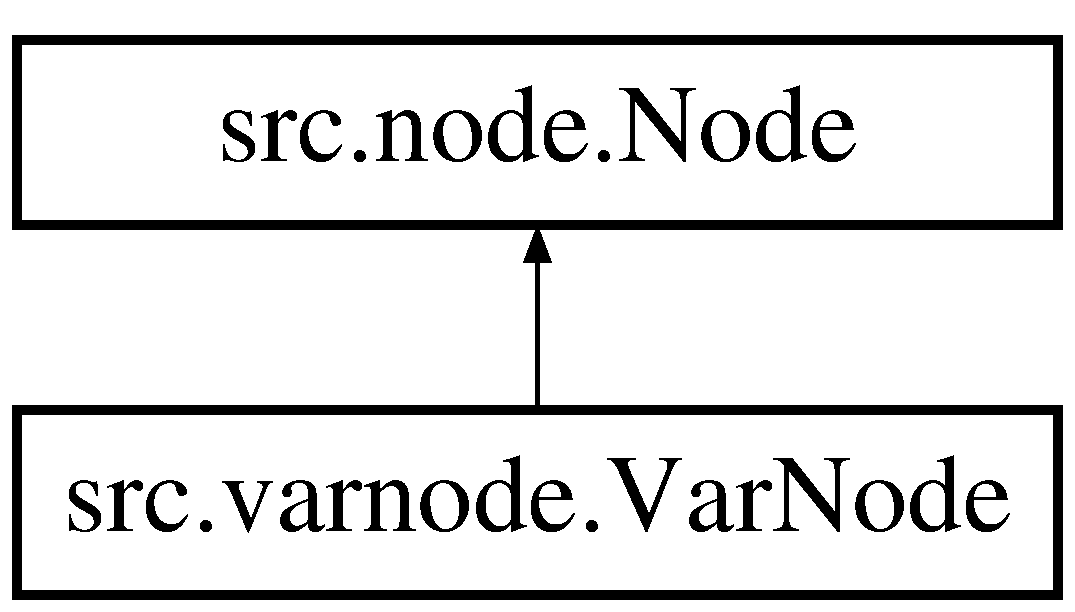
\includegraphics[height=2.000000cm]{classsrc_1_1varnode_1_1VarNode}
\end{center}
\end{figure}
\subsection*{Public Member Functions}
\begin{DoxyCompactItemize}
\item 
\mbox{\Hypertarget{classsrc_1_1varnode_1_1VarNode_aa630ffa27288975dd6c09233f38b2eb9}\label{classsrc_1_1varnode_1_1VarNode_aa630ffa27288975dd6c09233f38b2eb9}} 
def {\bfseries \+\_\+\+\_\+init\+\_\+\+\_\+} (self, name)
\item 
\mbox{\Hypertarget{classsrc_1_1varnode_1_1VarNode_ae238bcc420623c7c3df9327230b5d541}\label{classsrc_1_1varnode_1_1VarNode_ae238bcc420623c7c3df9327230b5d541}} 
def {\bfseries \+\_\+\+\_\+hash\+\_\+\+\_\+} (self)
\item 
\mbox{\Hypertarget{classsrc_1_1varnode_1_1VarNode_a78e85917702c2a35f57600c7f70d1844}\label{classsrc_1_1varnode_1_1VarNode_a78e85917702c2a35f57600c7f70d1844}} 
def {\bfseries \+\_\+\+\_\+eq\+\_\+\+\_\+} (self, other)
\item 
\mbox{\Hypertarget{classsrc_1_1varnode_1_1VarNode_ad4bdffd574d8d62c34efa3bd7943880e}\label{classsrc_1_1varnode_1_1VarNode_ad4bdffd574d8d62c34efa3bd7943880e}} 
def {\bfseries simplifyed} (self)
\item 
\mbox{\Hypertarget{classsrc_1_1varnode_1_1VarNode_a8ba0baacf1dd39e9126df15d5e573e9d}\label{classsrc_1_1varnode_1_1VarNode_a8ba0baacf1dd39e9126df15d5e573e9d}} 
def {\bfseries formatted} (self)
\item 
\mbox{\Hypertarget{classsrc_1_1varnode_1_1VarNode_a6aef19d72f67559cd9eac6078f168cf2}\label{classsrc_1_1varnode_1_1VarNode_a6aef19d72f67559cd9eac6078f168cf2}} 
def {\bfseries contains} (self, value)
\item 
\mbox{\Hypertarget{classsrc_1_1varnode_1_1VarNode_a819734f6e491de3c0702935e68e4b667}\label{classsrc_1_1varnode_1_1VarNode_a819734f6e491de3c0702935e68e4b667}} 
def {\bfseries contains\+\_\+unknown} (self)
\item 
\mbox{\Hypertarget{classsrc_1_1varnode_1_1VarNode_a004861059242e634e92e27635bfbf305}\label{classsrc_1_1varnode_1_1VarNode_a004861059242e634e92e27635bfbf305}} 
def {\bfseries latex} (self)
\end{DoxyCompactItemize}
\subsection*{Public Attributes}
\begin{DoxyCompactItemize}
\item 
\mbox{\Hypertarget{classsrc_1_1varnode_1_1VarNode_a1b645d6a685c2340eed9d37594f96de2}\label{classsrc_1_1varnode_1_1VarNode_a1b645d6a685c2340eed9d37594f96de2}} 
{\bfseries name}
\end{DoxyCompactItemize}


The documentation for this class was generated from the following file\+:\begin{DoxyCompactItemize}
\item 
src/varnode.\+py\end{DoxyCompactItemize}

%--- End generated contents ---

% Index
\backmatter
\newpage
\phantomsection
\clearemptydoublepage
\addcontentsline{toc}{chapter}{Index}
\printindex

\end{document}
